\documentclass[tikz,border=20pt]{standalone}
\usepackage{tikz}
\usetikzlibrary{shapes.geometric, arrows.meta, positioning, calc, fit, backgrounds}
\begin{document}
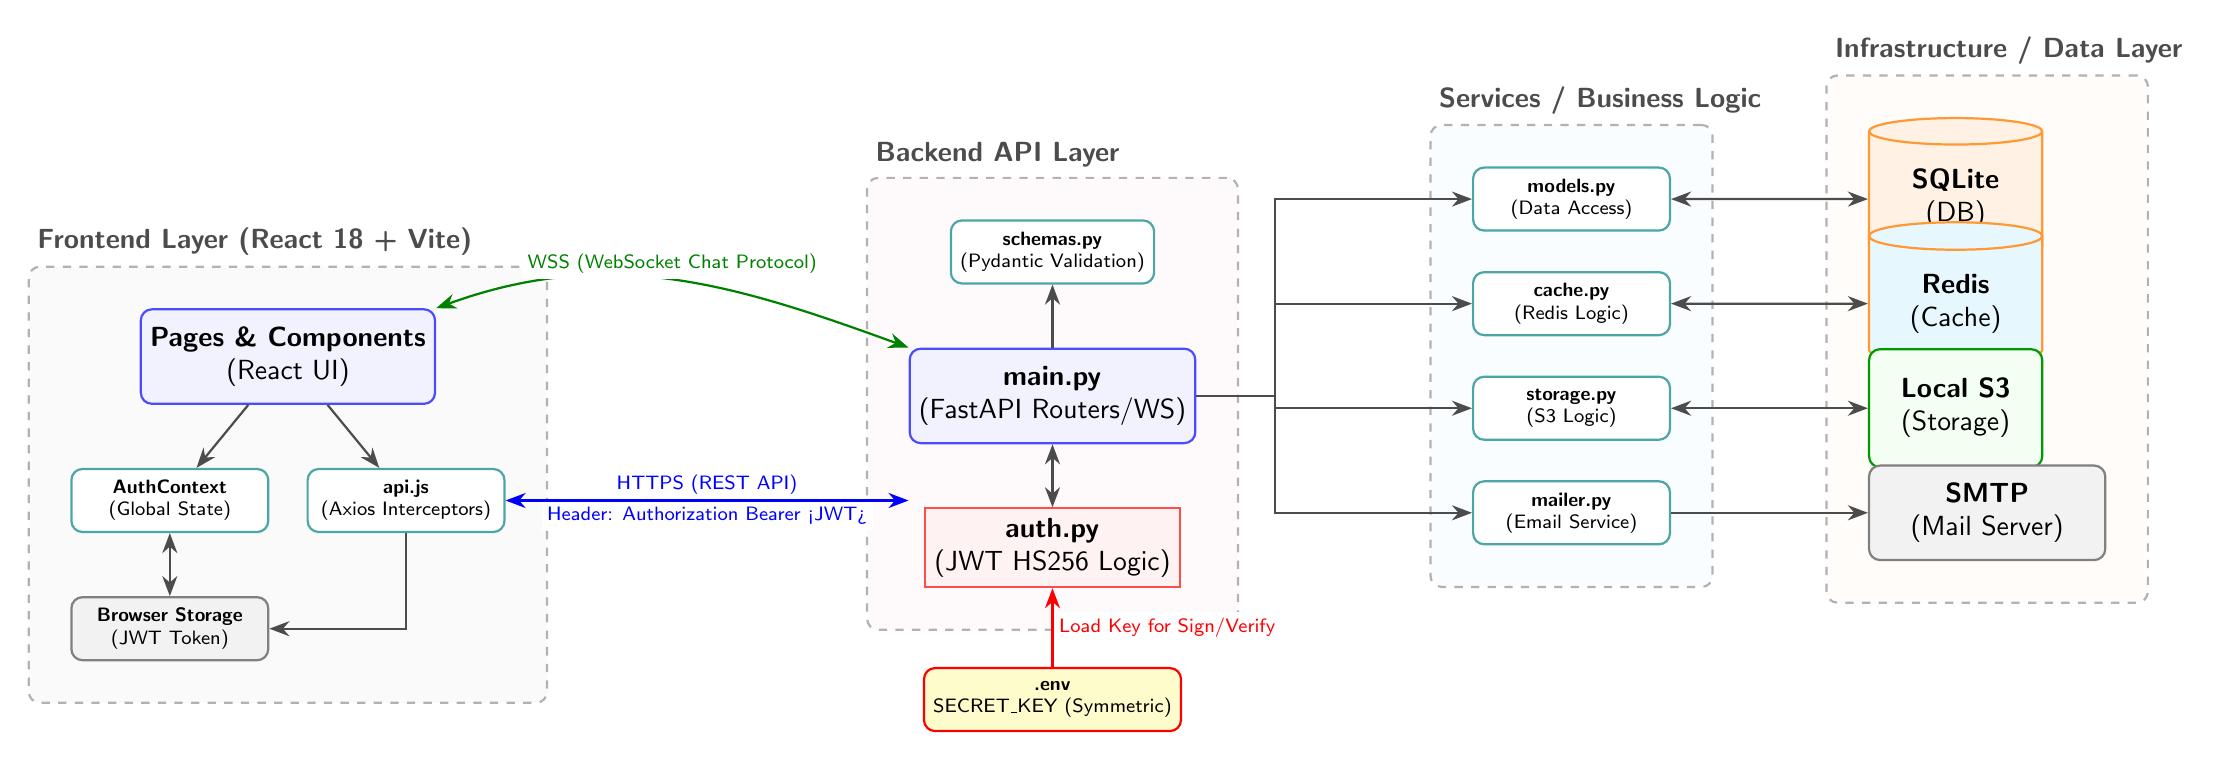
\begin{tikzpicture}[
    node distance=1.2cm and 2.5cm,
    every node/.style={font=\sffamily, align=center},
    layer/.style={rectangle, draw=black!30, dashed, thick, inner sep=15pt, rounded corners, fill=black!2},
    comp/.style={rectangle, draw=blue!70, fill=blue!5, thick, rounded corners, minimum width=3cm, minimum height=1.2cm},
    subcomp/.style={rectangle, draw=teal!70, fill=white, thick, rounded corners, minimum width=2.5cm, minimum height=0.8cm, font=\scriptsize\sffamily},
    db/.style={cylinder, draw=orange!80, thick, aspect=0.25, minimum height=1.8cm, minimum width=2.2cm, shape border rotate=90, fill=orange!10},
    storage/.style={rectangle, draw=green!60!black, fill=green!5, thick, rounded corners, minimum width=2.2cm, minimum height=1.5cm},
    auth/.style={rectangle, draw=red!70, fill=red!5, thick, minimum width=3cm, minimum height=1cm},
    arrow/.style={-{Stealth[scale=1.1]}, thick, draw=black!70},
    bidir/.style={<->, >={Stealth[scale=1.1]}, thick, draw=black!70},
    lbl/.style={font=\scriptsize\sffamily, fill=white, inner sep=2pt}
]

% ================= FRONTEND LAYER =================
\node[comp] (pages) {\textbf{Pages \& Components}\\(React UI)};
\node[subcomp, below=0.8cm of pages, xshift=-1.5cm] (authctx) {\textbf{AuthContext}\\(Global State)};
\node[subcomp, below=0.8cm of pages, xshift=1.5cm] (apijs) {\textbf{api.js}\\(Axios Interceptors)};
\node[subcomp, draw=gray, fill=gray!10, below=0.8cm of authctx] (localstorage) {\textbf{Browser Storage}\\(JWT Token)};

\draw[arrow] (pages) -- (authctx);
\draw[arrow] (pages) -- (apijs);
\draw[bidir] (authctx) -- (localstorage);
\draw[arrow] (apijs) |- (localstorage);

\begin{scope}[on background layer]
    \node[layer, fit=(pages) (authctx) (apijs) (localstorage)] (frontend) {};
    \node[anchor=south west, font=\sffamily\bfseries, color=black!70] at (frontend.north west) {Frontend Layer (React 18 + Vite)};
\end{scope}

% ================= BACKEND API LAYER =================
\node[comp, right=6cm of pages, yshift=-0.5cm] (main) {\textbf{main.py}\\(FastAPI Routers/WS)};
\node[subcomp, above=0.8cm of main] (schemas) {\textbf{schemas.py}\\(Pydantic Validation)};
\node[auth, below=0.8cm of main] (authpy) {\textbf{auth.py}\\(JWT HS256 Logic)};

\draw[arrow] (main) -- (schemas);
\draw[bidir] (main) -- (authpy);

\begin{scope}[on background layer]
    \node[layer, fill=purple!2, fit=(main) (schemas) (authpy)] (api_layer) {};
    \node[anchor=south west, font=\sffamily\bfseries, color=black!70] at (api_layer.north west) {Backend API Layer};
\end{scope}

% ================= BACKEND SERVICES LAYER =================
\node[subcomp, right=3.5cm of main, yshift=2.5cm] (models) {\textbf{models.py}\\(Data Access)};
\node[subcomp, below=0.5cm of models] (cache) {\textbf{cache.py}\\(Redis Logic)};
\node[subcomp, below=0.5cm of cache] (storagepy) {\textbf{storage.py}\\(S3 Logic)};
\node[subcomp, below=0.5cm of storagepy] (mailer) {\textbf{mailer.py}\\(Email Service)};

\draw[arrow] (main.east) -- +(1cm,0) |- (models.west);
\draw[arrow] (main.east) -- +(1cm,0) |- (cache.west);
\draw[arrow] (main.east) -- +(1cm,0) |- (storagepy.west);
\draw[arrow] (main.east) -- +(1cm,0) |- (mailer.west);

\begin{scope}[on background layer]
    \node[layer, fill=cyan!2, fit=(models) (cache) (storagepy) (mailer)] (services) {};
    \node[anchor=south west, font=\sffamily\bfseries, color=black!70] at (services.north west) {Services / Business Logic};
\end{scope}

% ================= INFRASTRUCTURE LAYER =================
\node[db, right=2.5cm of models] (sqlite) {\textbf{SQLite}\\(DB)};
\node[db, fill=cyan!10, right=2.5cm of cache] (redisdb) {\textbf{Redis}\\(Cache)};
\node[storage, right=2.5cm of storagepy] (s3db) {\textbf{Local S3}\\(Storage)};
\node[comp, fill=gray!10, draw=gray, right=2.5cm of mailer] (smtp) {\textbf{SMTP}\\(Mail Server)};

\draw[bidir] (models) -- (sqlite);
\draw[bidir] (cache) -- (redisdb);
\draw[bidir] (storagepy) -- (s3db);
\draw[arrow] (mailer) -- (smtp);

\begin{scope}[on background layer]
    \node[layer, fill=orange!2, fit=(sqlite) (redisdb) (s3db) (smtp)] (infra) {};
    \node[anchor=south west, font=\sffamily\bfseries, color=black!70] at (infra.north west) {Infrastructure / Data Layer};
\end{scope}

% ================= KEY MANAGEMENT & COMMUNICATION =================
\node[subcomp, fill=yellow!20, draw=red, thick, below=1cm of authpy] (env) {\textbf{.env}\\SECRET\_KEY (Symmetric)};
\draw[arrow, red, thick] (env) -- node[right, lbl] {Load Key for Sign/Verify} (authpy);

% Client to Server communication
\draw[bidir, thick, blue] (apijs.east) -- node[above, lbl, text=blue] {HTTPS (REST API)} node[below, lbl, text=blue] {Header: Authorization Bearer <JWT>} (main.west |- apijs);

\draw[bidir, thick, green!50!black] (pages.north east) to[out=20, in=160] node[above, lbl, text=green!50!black] {WSS (WebSocket Chat Protocol)} (main.north west);

\end{tikzpicture}
\end{document}
